\chapter{Supplementary Information for Chapter~\ref{ch:Raman}}
\label{appendix: Raman}
\acresetall

\section{Thin Film Fabrication via Physical Vapor Deposition}
\label{Raman:Appendix:sec:ThinFilmFabricationViaPVD}

\begin{figure}[t]
  \centering
  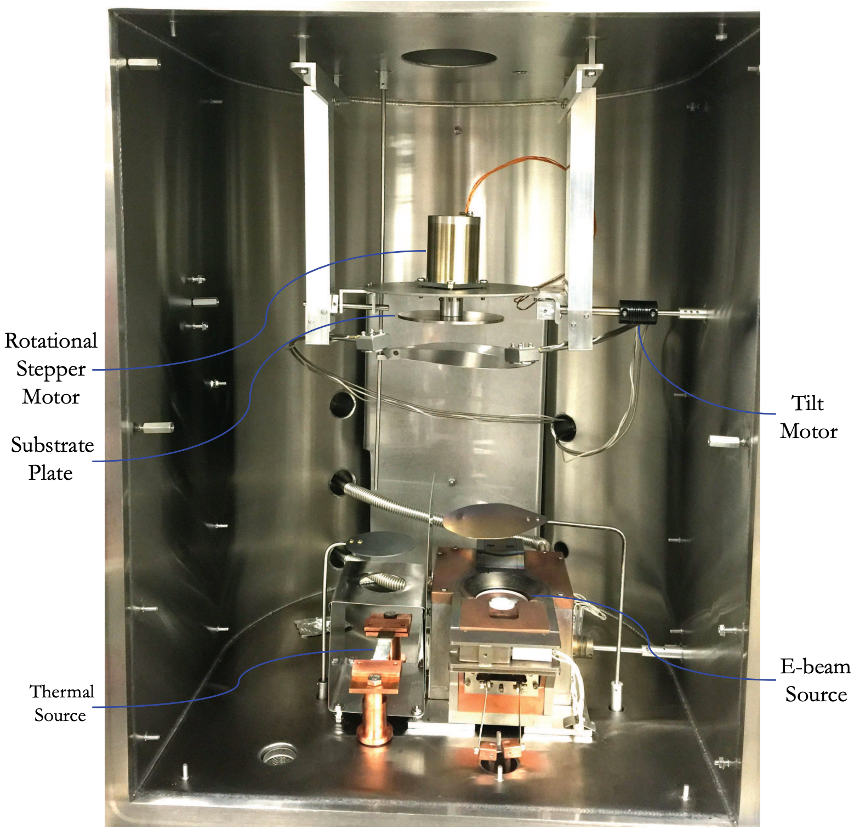
\includegraphics[width=\textwidth]{figs/4-Raman/DepositionChamber.png}
  \caption{Dr. John Gibbs Nanotechnology Laboratory \ac{PVD} chamber.}
  \label{fig:Raman:DepositionChamber}
\end{figure}

\begin{figure}[t]
  \centering
  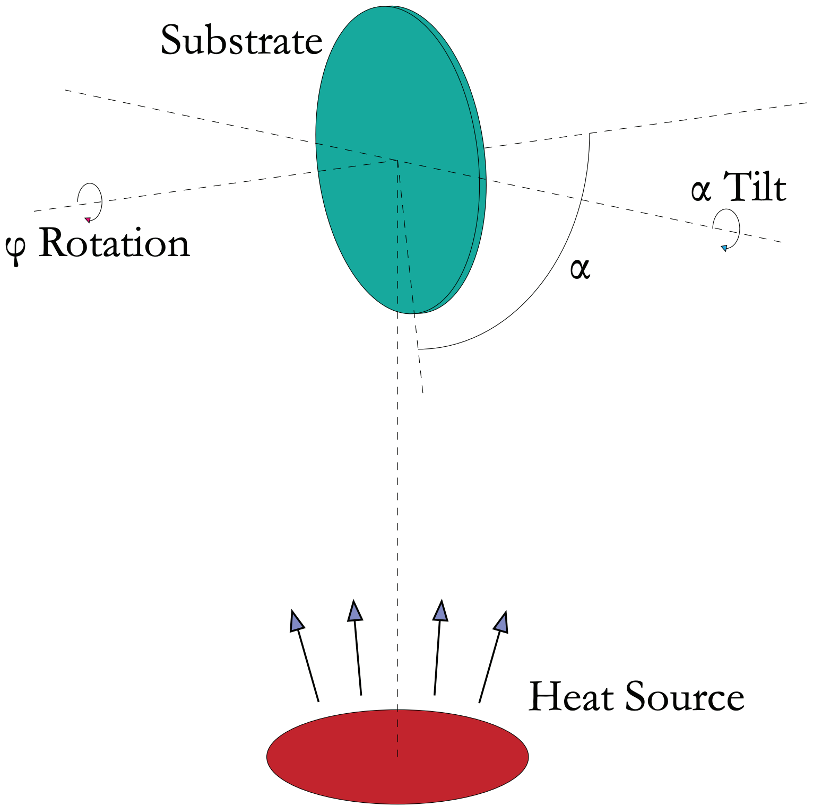
\includegraphics[width=.8\textwidth]{figs/4-Raman/GLAD.png}
  \caption{Diagram showing Glancing Angle Deposition (\acs{GLAD}), a technique which offers the ability to fabricate complex thin films and nanostructures such as rods and helices via programatic control of deposition parameters and substrate degrees of freedom.}
  \label{fig:Raman:GLAD}
\end{figure}

\begin{figure}[t]
  \centering
  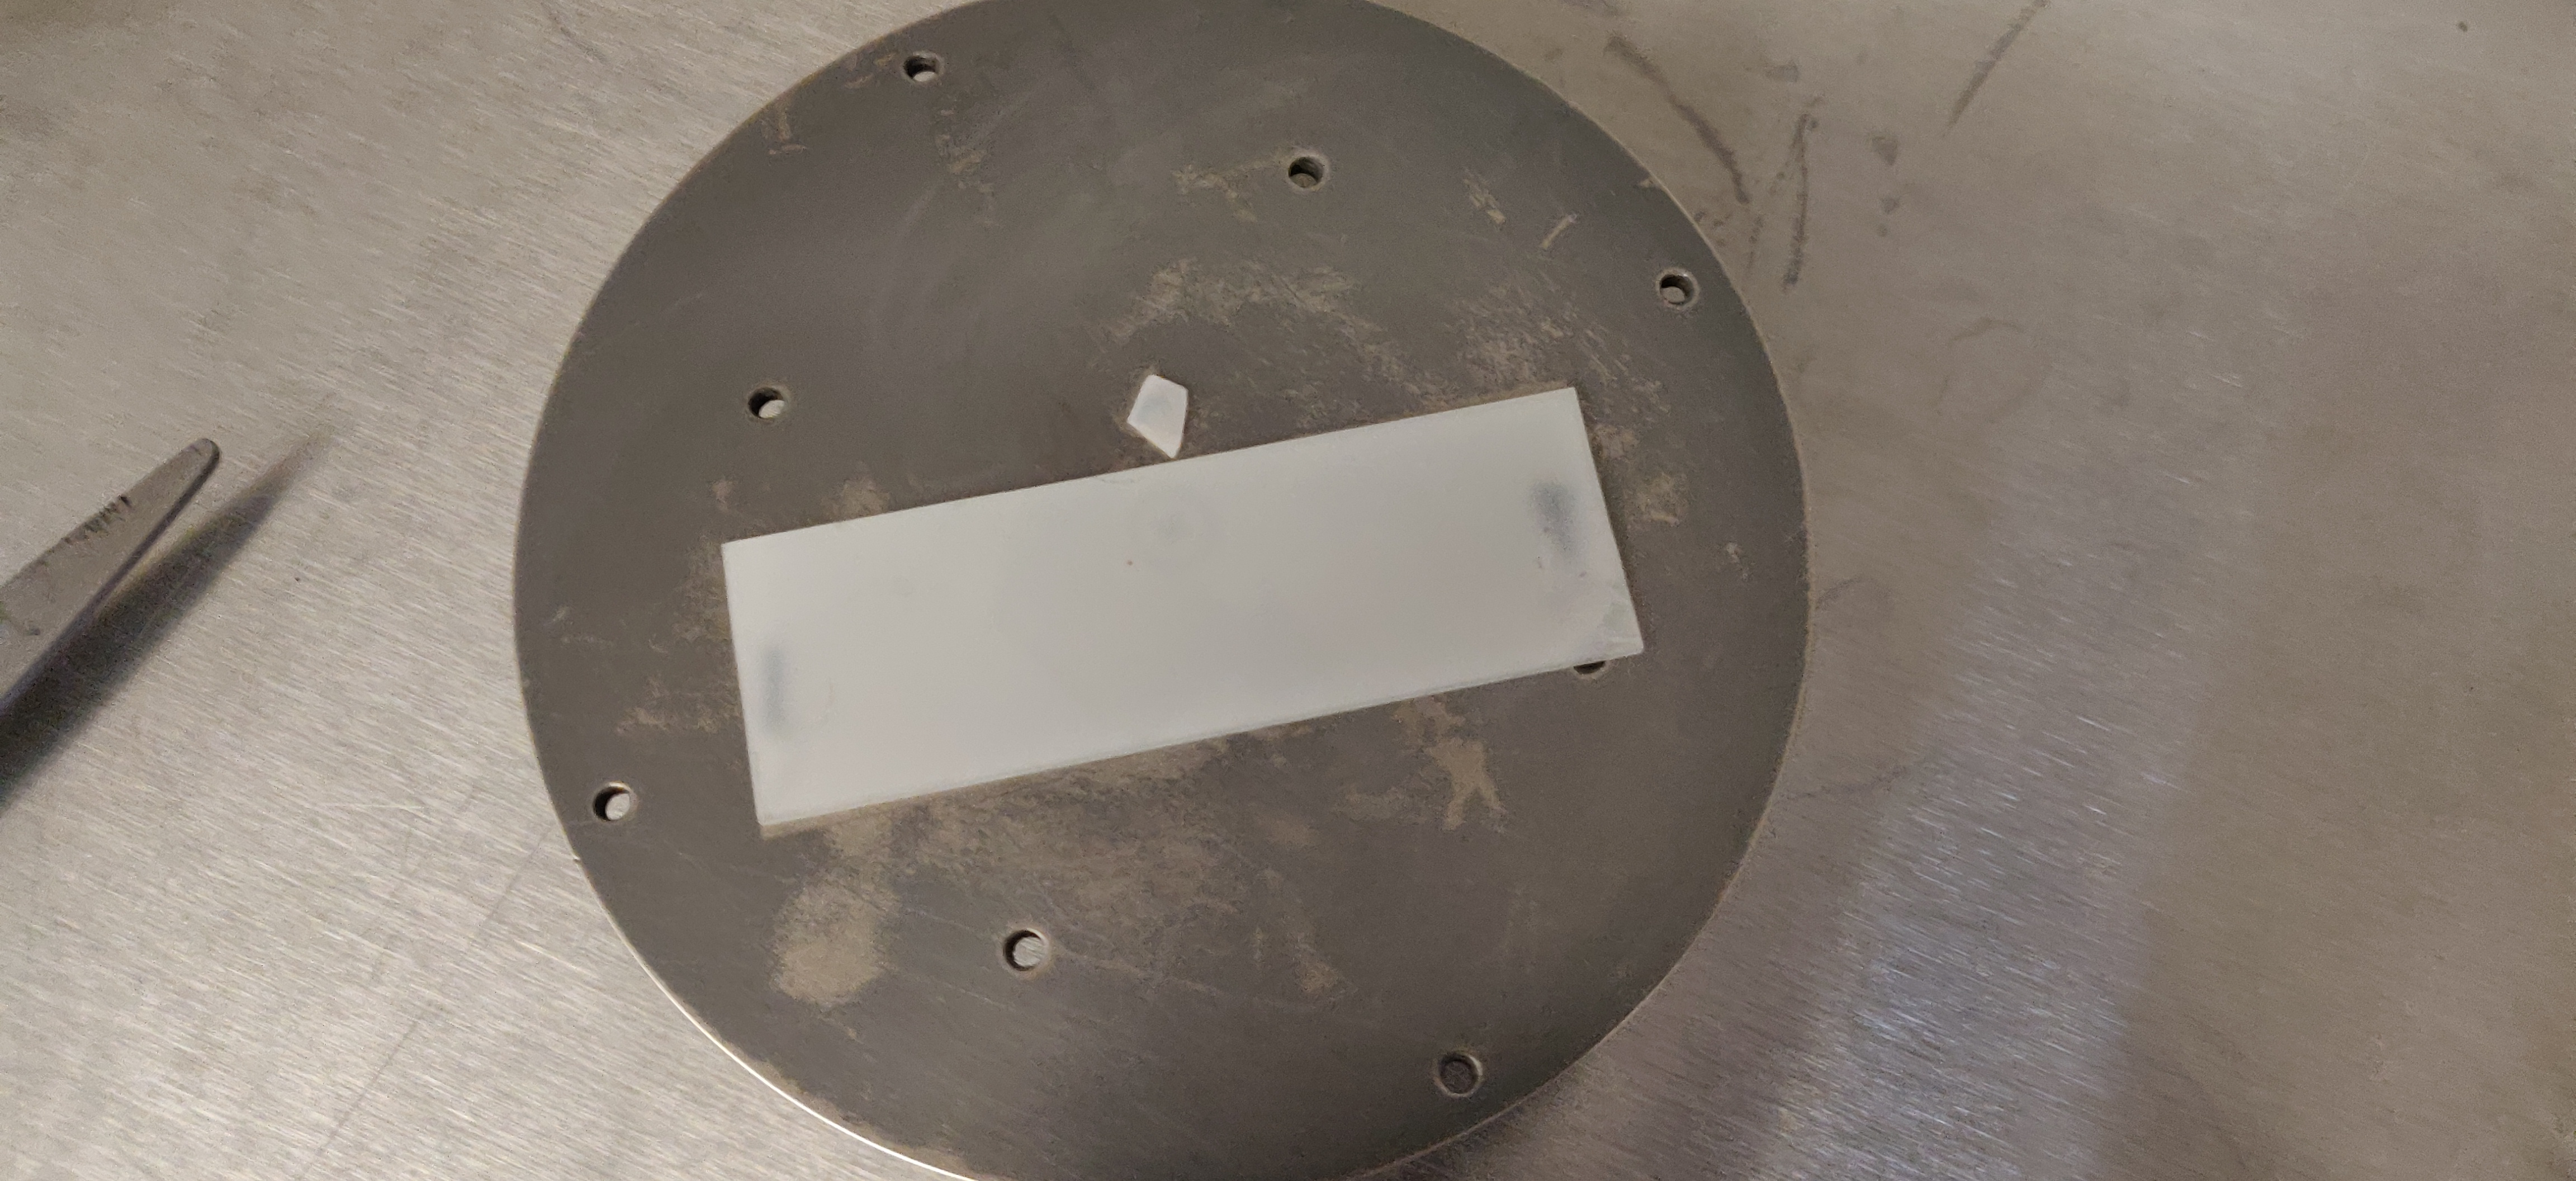
\includegraphics[width=\textwidth]{figs/4-Raman/slide-with-TeO2-film-on-substrate.jpeg}
  \caption{Photograph of \ce{TeO2} thin film deposited via \ac{PVD} onto glass slide substrate.}%was this deposited TeO2 or Te then annealed?
  \label{fig:Raman:TeO2onSubstrate}
\end{figure}

\begin{figure}[t]
  \centering
  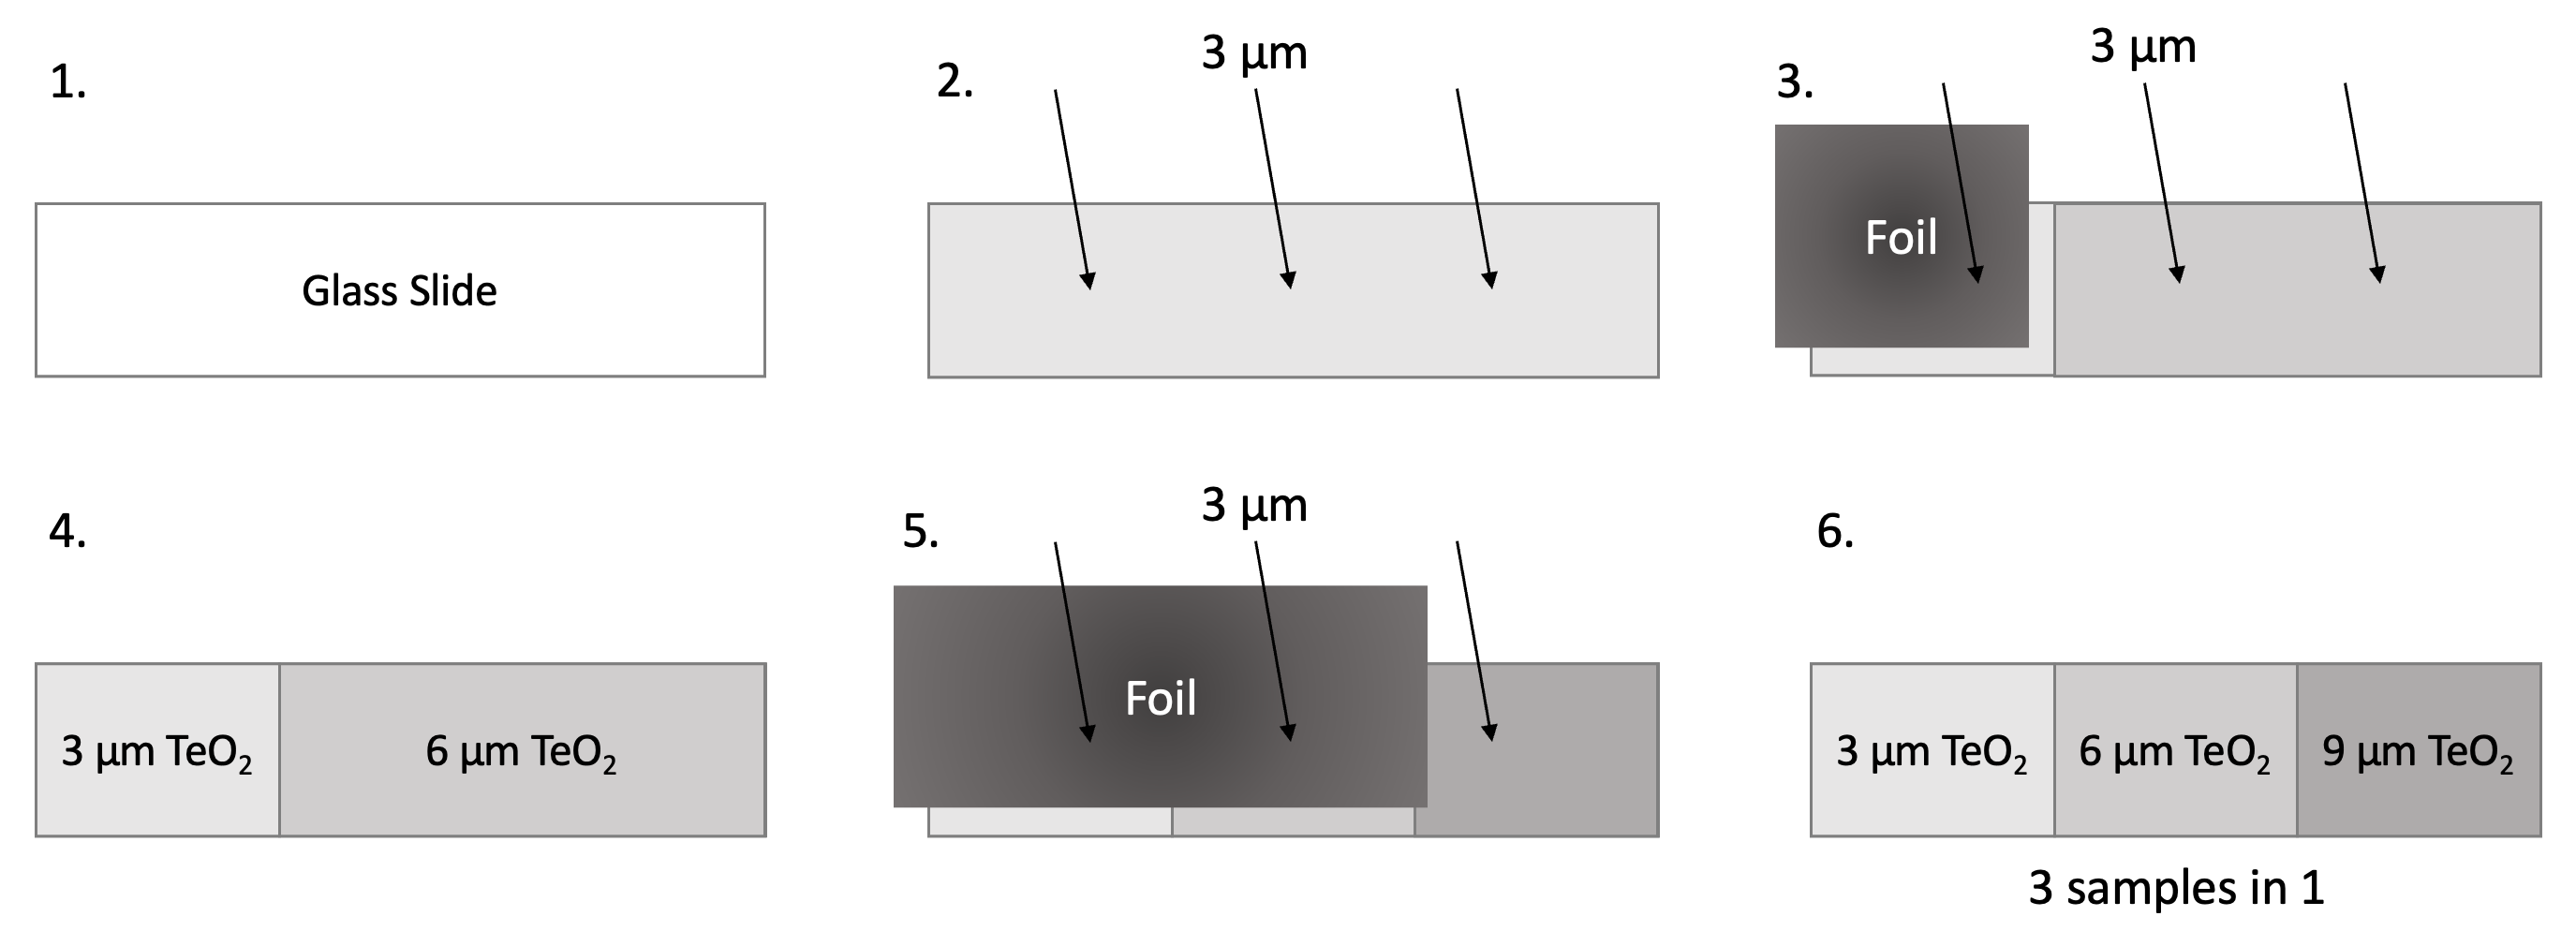
\includegraphics[width=\textwidth]{figs/4-Raman/3TeO2SamplesIn1.png}
  \caption{Diagram showing the multi-deposition process for fabricating \ce{Te} thin films of three thicknesses on one glass slide sample using \ac{PVD}.}
  \label{fig:Raman:3in1}
\end{figure}

\begin{figure}[t]
    \centering
    \begin{subfigure}[b]{0.49\textwidth}
        \centering
        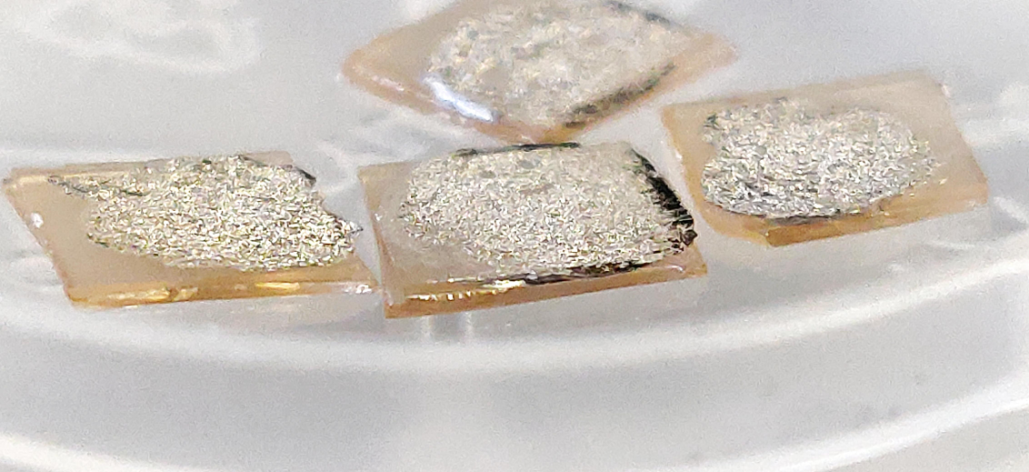
\includegraphics[width=\textwidth]{figs/4-Raman/CINTSamples.png}
        \caption{}
        \label{fig:Raman:CINTSamplesFacedown}
    \end{subfigure}
    \hfill
    \begin{subfigure}[b]{0.49\textwidth}
        \centering
        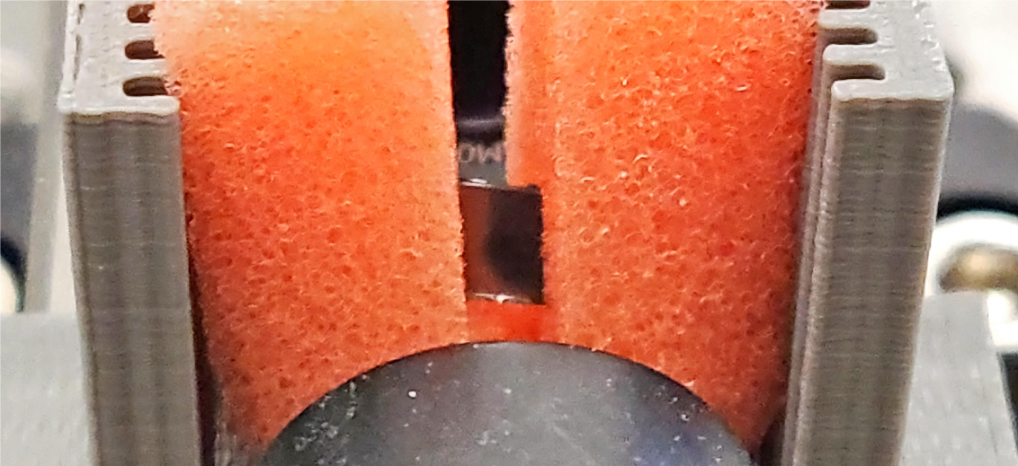
\includegraphics[width=\textwidth]{figs/4-Raman/TeCINTinFoam.png}
        \caption{}
        \label{fig:Raman:TeCINTinFoam}
    \end{subfigure}
    \caption{(\ref{fig:Raman:CINTSamplesFacedown}) Photograph of sapphire substrates primed with \SI{20}{\nano\meter} \ce{Se} adhesion layer. Critical surface is layed face down in curved-bottom protective container. (\ref{fig:Raman:TeCINTinFoam}) \SI{500}{\nano\meter} \ce{Te} thin film sample secured in beam path of \acl{CoBS}. \ce{Te} is deposited ontop of the \SI{20}{\nano\meter} \ce{Se} adhesion layer for ablation prevention.}
    \label{fig:Raman:CINTSamples}
\end{figure}

\section{Fiber-Chip-Fiber Waveguide Optical Alignment}
\label{Raman:Appendix:sec:WaveguideAlignment}

\begin{figure}[t]
  \centering
  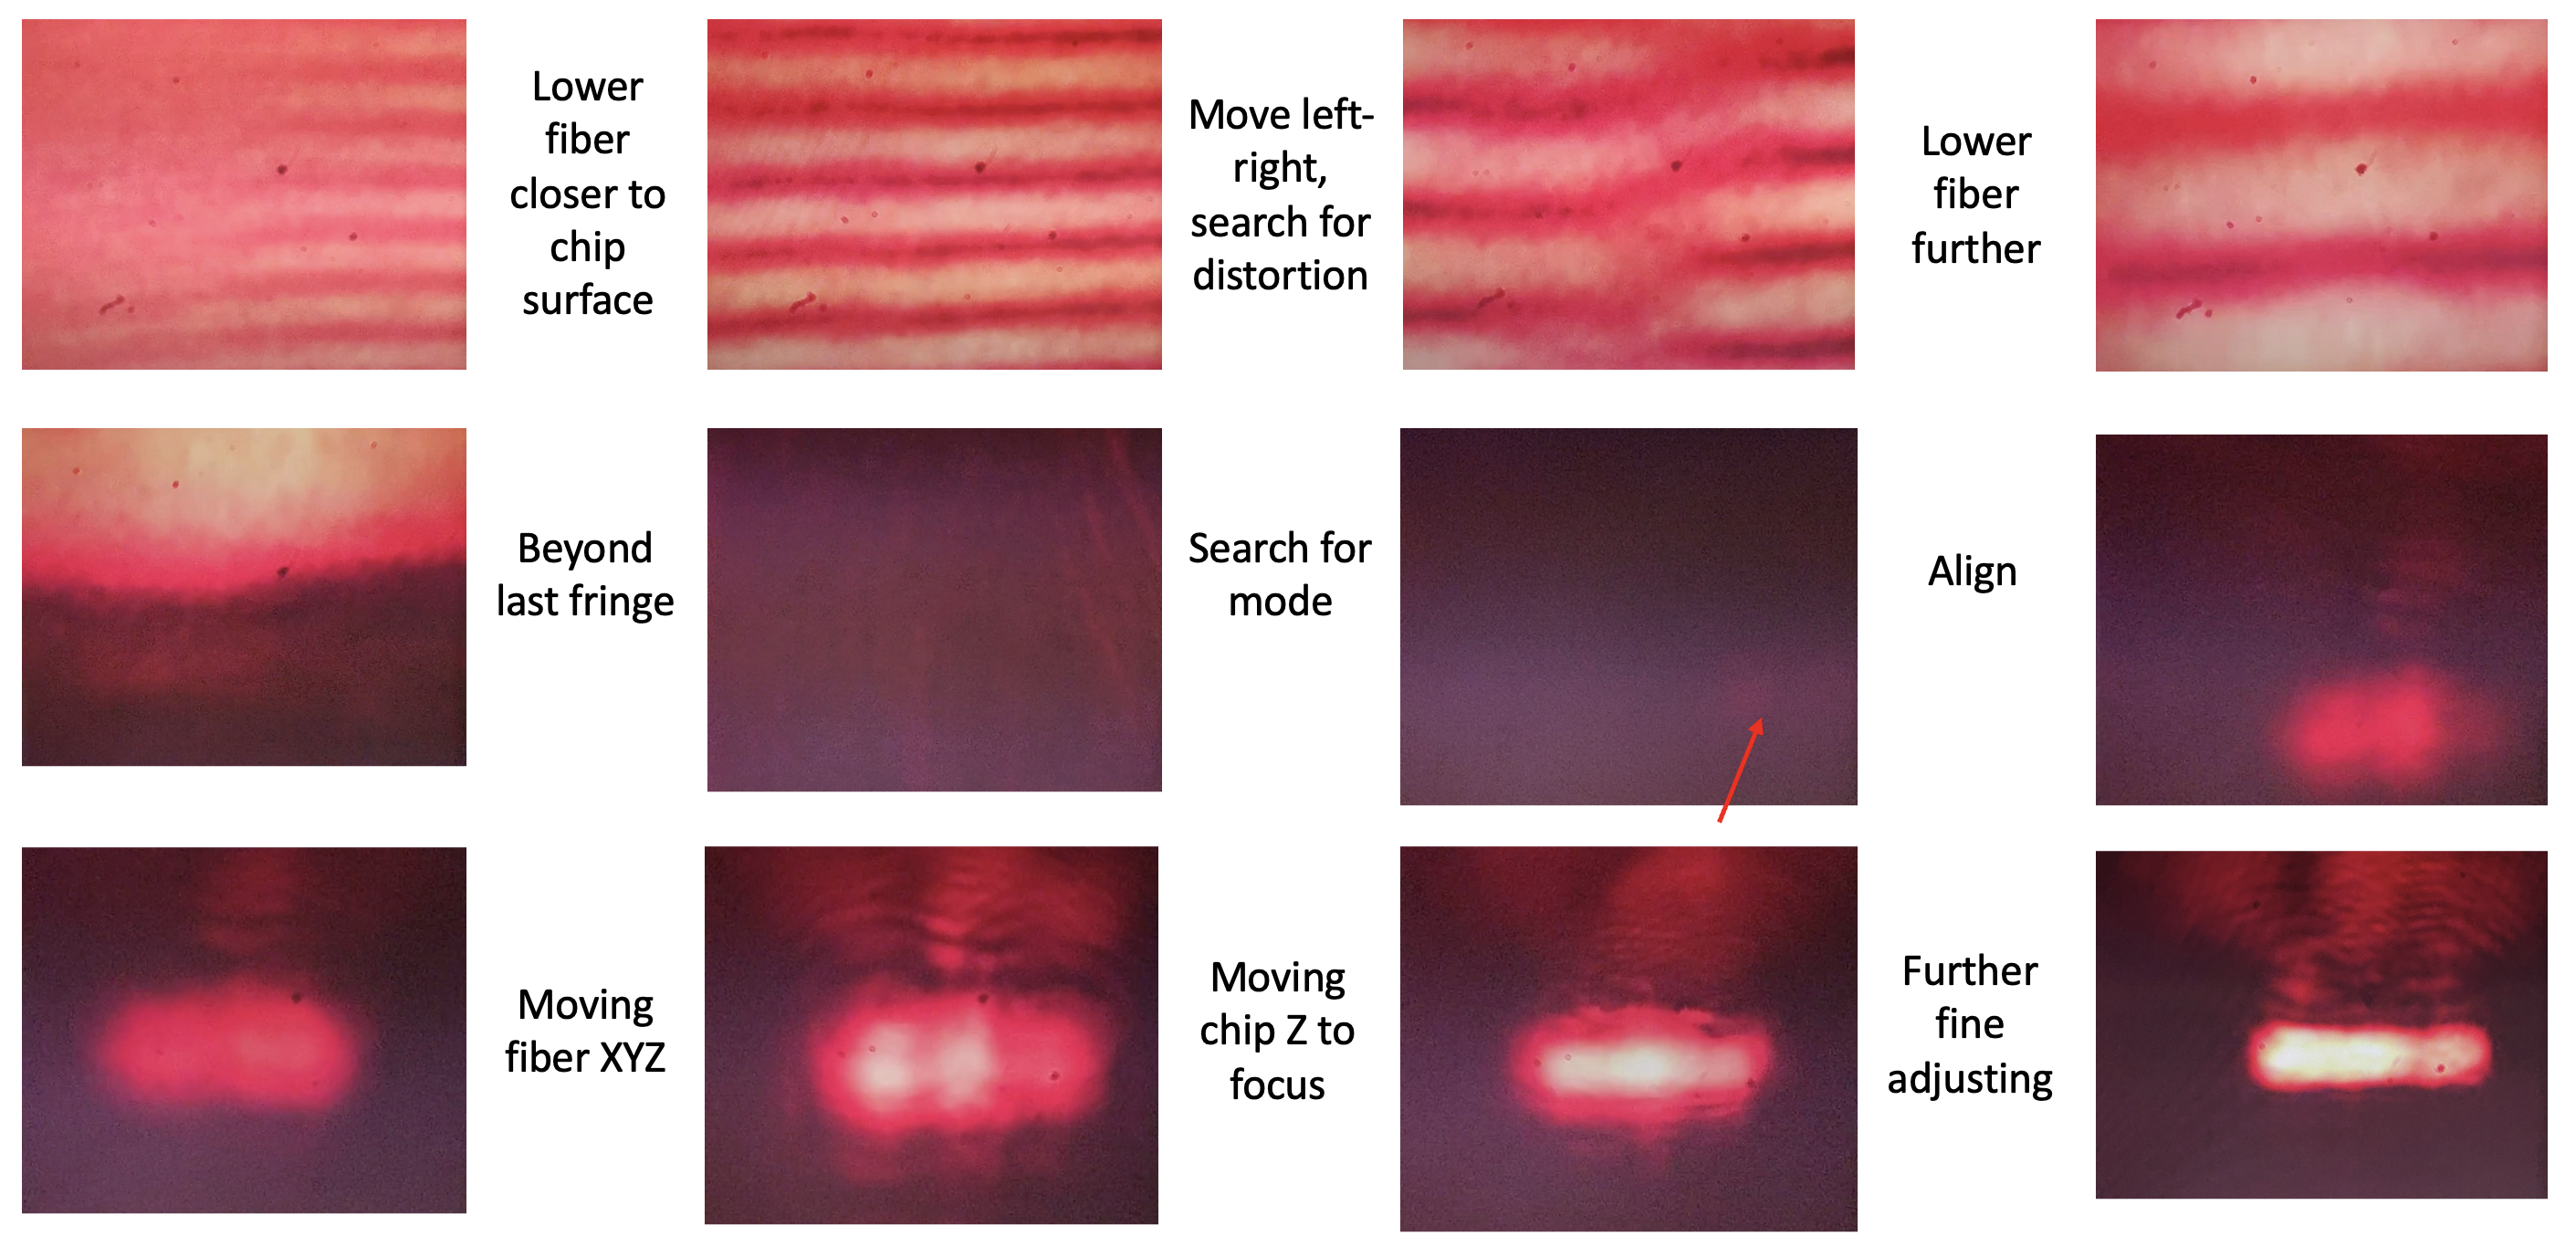
\includegraphics[width=\textwidth]{figs/4-Raman/WaveguideAlignmentCameraFringePattern.png}
  \caption{Step-by-step visuals from camera in process of aligning the input optical fiber to the chip waveguide, read from top left to bottom right.}
  \label{fig:Raman:WaveguideAlignmentCameraFringePattern}
\end{figure}

\section{Chip Waveguide Case Study~A: Thermal Effect on Brillouin Frequency Shift}
\label{Raman:Appendix:sec:CaseStudyAThermal}

froze the lab

\section{Chip Waveguide Case Study~B: Pump-Probe Detuning Effect on Scattered Power}
\label{Raman:Appendix:sec:CaseStudyBDetuning}

P-Pr detuning
